% !TeX spellcheck = de_DE
% !TeX root = kristallographie_skript.tex
\begin{sheet}

\begin{problem}
Schaue dir die Bilder, gedacht als 2D Kristalle, auf den folgenden Seiten an.
\begin{subproblem}
Bestimme möglichst viele wesentlich verschiedene Symmetrien
\end{subproblem}
\begin{subproblem}
Finde mögliche Basiszellen
\end{subproblem}
\end{problem}

\begin{problem}[difficulty={fortgeschritten}]
Das Prinzip, mit dem wir die Operation von $\Aut(\Lambda)$ auf einem Drei-Torus konstruiert haben, lässt sich wie folgt abstrahieren und verallgemeinern:

Gegeben eine Gruppe $G$, einen Normalteiler $N\unlhd G$ und eine Operation von $G$ auf $\Omega$, dann operiert $G/N$ auf dem Bahnenraum $\Omega/N$ wie folgt:
\[{^{gN} B} := {^g B} := \Set{{^g \omega} | \omega\in B}\]
\begin{subproblem}[difficulty={einfach}]
Man zeige, dass dies wohldefiniert ist, d.h.
\[\forall g,h\in G, B\in\Omega/N: gN=hN \implies {^g B} = {^h B}\]
\end{subproblem}
\begin{subproblem}[difficulty={mittel}]
Man überlege sich, dass dies genau unsere Konstruktion mit dem 3-Torus ergibt, wenn wir $G=\Aut(\Lambda)$ auf $\Omega=\IR^3$ operieren lassen und $N=\mathcal{T}$ betrachten. Hinweis: Man überlege sich zuerst, wieso der 3-Torus genau $\IR / \mathcal{T}$ ist.
\end{subproblem}
\end{problem}

\begin{problem}[difficulty={leicht bis mittel}]
Finde zu jedem der sieben Gittersysteme ein Translationsgitter, das in dieses Gittersystem fällt.
\end{problem}

\begin{problem}
	Andrea und Johannes haben Polyeder mitgebracht. 
	\begin{subproblem}
		Bestimme das Hermann-Mauguin-Symbol für einige Polyeder. Schreibe das Symbol auf ein Stück Papier und lege es zusammengefaltet in die Tischmitte.
	\end{subproblem}
	\begin{subproblem}
		In der Tischmitte sollten einige Zettel Papier liegen. Nimm dir einige (aber nicht die eigenen) und ordne den darauf notierten Hermann-Mauguin-Symbolen ihr jeweiliges Gittersystem zu.
	\end{subproblem}
	\begin{subproblem}[difficulty={mittel}]
		Bestimme die Tracht der Kristalle, die durch von dir die gezogenen Hermann-Mauguin-Symbole beschrieben werden.
	\end{subproblem}
	
\end{problem}
\begin{problem}[difficulty={sehr leicht}]
	Lilly hat einige Basiszellen auf ihrem Laptop mitgebracht, schaue sie dir an.
\end{problem}
\includepdf[pages=3-8, nup=1x2,angle=90]{../Übungen/GroupSymmetryExercises/TranslationsvektorenGitter/Aufgabenblatt01_1}
\includepdf[pages=2-5, nup=1x2,angle=90]{../Übungen/GroupSymmetryExercises/TranslationsvektorenGitter/Aufgabenblatt01_2}

\begin{problem}
	Gegeben (im Anschluss an den Bildern der 2D-Kristalle) ist eine Projektion einer Elementarzelle einer Raumgruppe auf die Ebene aufgespannt durch die ersten zwei Basisvektoren $a,b$. Die Position eines Atoms ist durch einen schraffierten Kreis gekennzeichnet. Einige andere Positionen sind zur Unterstützung mit A bis S benannt.
	\begin{subproblem}
	Zu welchem Gittersystem geho ̈rt die abgebildete Raumgruppe?
	\end{subproblem}
	\begin{subproblem}
	Was ist das Hermann-Mauguin-Symbol dieses Kristalls?
	\end{subproblem}
	\begin{subproblem}
	Welche der Positionen A bis S sind die anderen, symmetrieäquivalenten Positionen zum gegebenen Atoms (schraffierter Kreis)?
	Bemerkung: Wenn eine Symmetrieoperation eine Position außerhalb der gegebenen Elementarzelle erzeugt, bedenke, dass man diese stets durch ein ganzzahliges Vielfaches eines oder mehrerer Basisvektoren in die Elementarzelle zurücktransferieren kann.
	\end{subproblem}
	\begin{subproblem}
		Was sind die Höhen der anderen Atome in der Elementarzelle, wenn sich das gegebene Atom auf der Höhe $+z$ (mit $0 \leq z < \frac{1}{2}$) befindet?
	\end{subproblem}
\begin{figure}
\includepdf[pages=2, offset=0 -270]{../Übungen/GroupSymmetryExercises/vorwiegendRaumgruppe/Aufgabenblatt07}
\end{figure}

\end{problem}

%\includepdf[pages=2]{../Übungen/GroupSymmetryExercises/vorwiegendRaumgruppe/Aufgabenblatt07}

\end{sheet}